\documentclass{article}

\usepackage{graphicx}
\usepackage{amsmath}
\usepackage{siunitx}

\title{Mapping circuit to transfer function}
\author{Anderson Hsieh}
\date{August 5, 2026}

\begin{document}

\maketitle

\section{Questions Answered}
    \subsection{solving RC circuit : rc1}
    so we have a RC circuit, we find its transfer function 
    \begin{align*}
        H(s)&=\frac{V_{out}(s)}{V_{in}(s)}\\
        V_{out}(s)&=V_{in}(s)*\frac{Z_c}{Z_c+Z_R}\\
        V_{out}(s)&=V_{in}(s)*\frac{\frac{1}{sC}}{\frac{1}{sC}+R}\\
        H(s)&=\frac{\frac{1}{sC}}{\frac{1}{sC}+R}
    \end{align*}
    $V_{in}(s) = 1$ because input is a AC source with amplitude of 1\\
    say 
    \begin{align*}
        C = \SI{1}{\pico\farad} = \SI{1e-12}{\farad}, R = \SI{1}{\kilo\ohm} = \SI{1e3}{\ohm}
    \end{align*}

    so now to calculate for the -3dB frequency.\\
    The definition of -3dB frequency is :\\
    \begin{quote}
        \textit{The point where a circuit's output power drops to half of its maximum value}\\
    \end{quote}
    in other words :\\
    \begin{quote}
    \textit{The point where a circuit's output voltage drops to $\frac{1}{\sqrt{2}}$ of its maximum value}\\
    \end{quote}
    We are looking for the frequency where if we input a cosine wave at such frequency, aka multiply that input expression(say $V_{in}(s)$) with the transfer function H(s), we would get an expression of the $V_{out}(s)$ where 
    \begin{align}
        V_{out}(s) &= V_{in}(s) * |H(\text{frequency of max gain})| * \frac{1}{\sqrt{2}}\label{eq:1}\\
        \mathcal{L}\left\{cos(wt)\right\} &= \frac{s}{s^2 + \omega^2}
    \end{align}
    if $|H(\text{frequency of max gain})| = 1$\\
    @ -3dB frequency :
    \begin{align*}
        \frac{s}{s^2 + \omega^2} * H(s) = \frac{s}{s^2 + \omega^2} * \frac{1}{\sqrt{2}}
    \end{align*}
    looking at \eqref{eq:1} we can see that by looking for the -3dB frequency, we're basically looking for where
    \begin{quote}
        \textit{The point where a circuit's voltage gain drops to $\frac{1}{\sqrt{2}}$ of its maximum voltgae gain}\\
    \end{quote}

    now we can actually start calcualting the -3dB frequency. Because this is an RC cirucit, we know that the max gain frequency is at DC. 
    \begin{align*}
        |H(0)| &=\frac{\frac{1}{sC}}{\frac{1}{sC}+R} = \frac{1}{1+R*sC} = 1
    \end{align*}
    we're looking for the frequency where
    \begin{align}
        s &= j\omega\notag\\
        |H(s)| &= |H(0)| * \frac{1}{\sqrt{2}} = \frac{1}{\sqrt{2}} \approx 0.7071\notag\\
        |H(s)| &= |\frac{\frac{1}{sC}}{\frac{1}{sC}+R}|\notag\\
        \frac{1}{\sqrt{2}} &= |\frac{1}{1+R*sC}|\notag\\
        \frac{1}{\sqrt{2}} &= |\frac{1}{1+R*j\omega C}|\notag\\
        \frac{1}{\sqrt{2}} &= \frac{1}{|1+R*j\omega C|}\notag\\
        \frac{1}{\sqrt{2}} &= \frac{1}{\sqrt{1^2+(\omega RC)^2}}\notag\\
        \sqrt{1+(\omega RC)^2} &= \sqrt{2}\notag\\
        1+(\omega RC)^2 &= 2\notag\\
        (\omega RC)^2 &= 1\notag\\
        \omega RC &= 1\notag\\
        \omega &= 2\pi \omega f = \frac{1}{RC}\notag\\
        f_{-3dB} &= \frac{1}{2\pi RC}\label{eq:2}\\
        f_{-3dB} &= \frac{1}{2\pi * \SI{1e3}{\ohm} * \SI{1e-12}{\farad}}\notag\\
        f_{-3dB} &\approx \SI{159.15}{\mega\hertz}\notag
    \end{align}
    we saw equation \eqref{eq:2} is the well known cut off frequency expression for an RC circuit. Plugging our RC nubmers in we get
    \begin{align*}
        \frac{1}{RC} = \frac{1}{(\SI{1e3}{\ohm})(\SI{1e-12}{\farad})} = \SI{1e9}{\radian\per\second}\\
        f_{-3\mathrm{dB}} = \frac{\omega_{-3\mathrm{dB}}}{2\pi}=\frac{\SI{1e9}{\radian\per\second}}{2\pi} \approx \SI{159.15}{\mega\hertz}
    \end{align*}
    That reflects our SPICE simulation and Octave script\\
    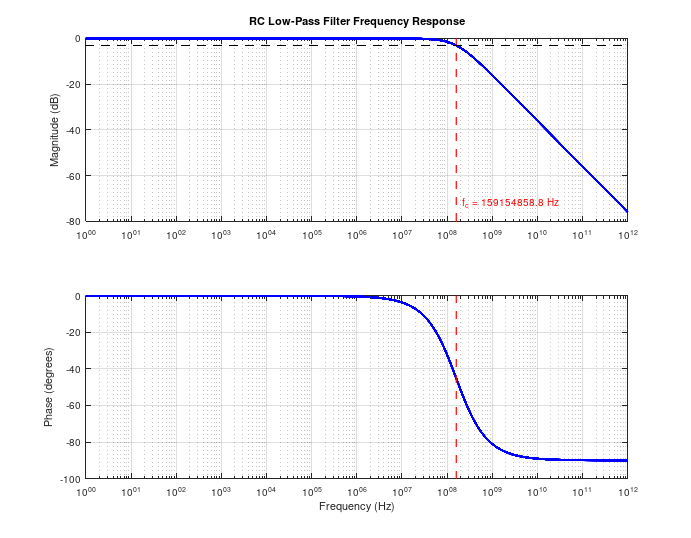
\includegraphics[width=\textwidth]{images/rc1_octave.png}
    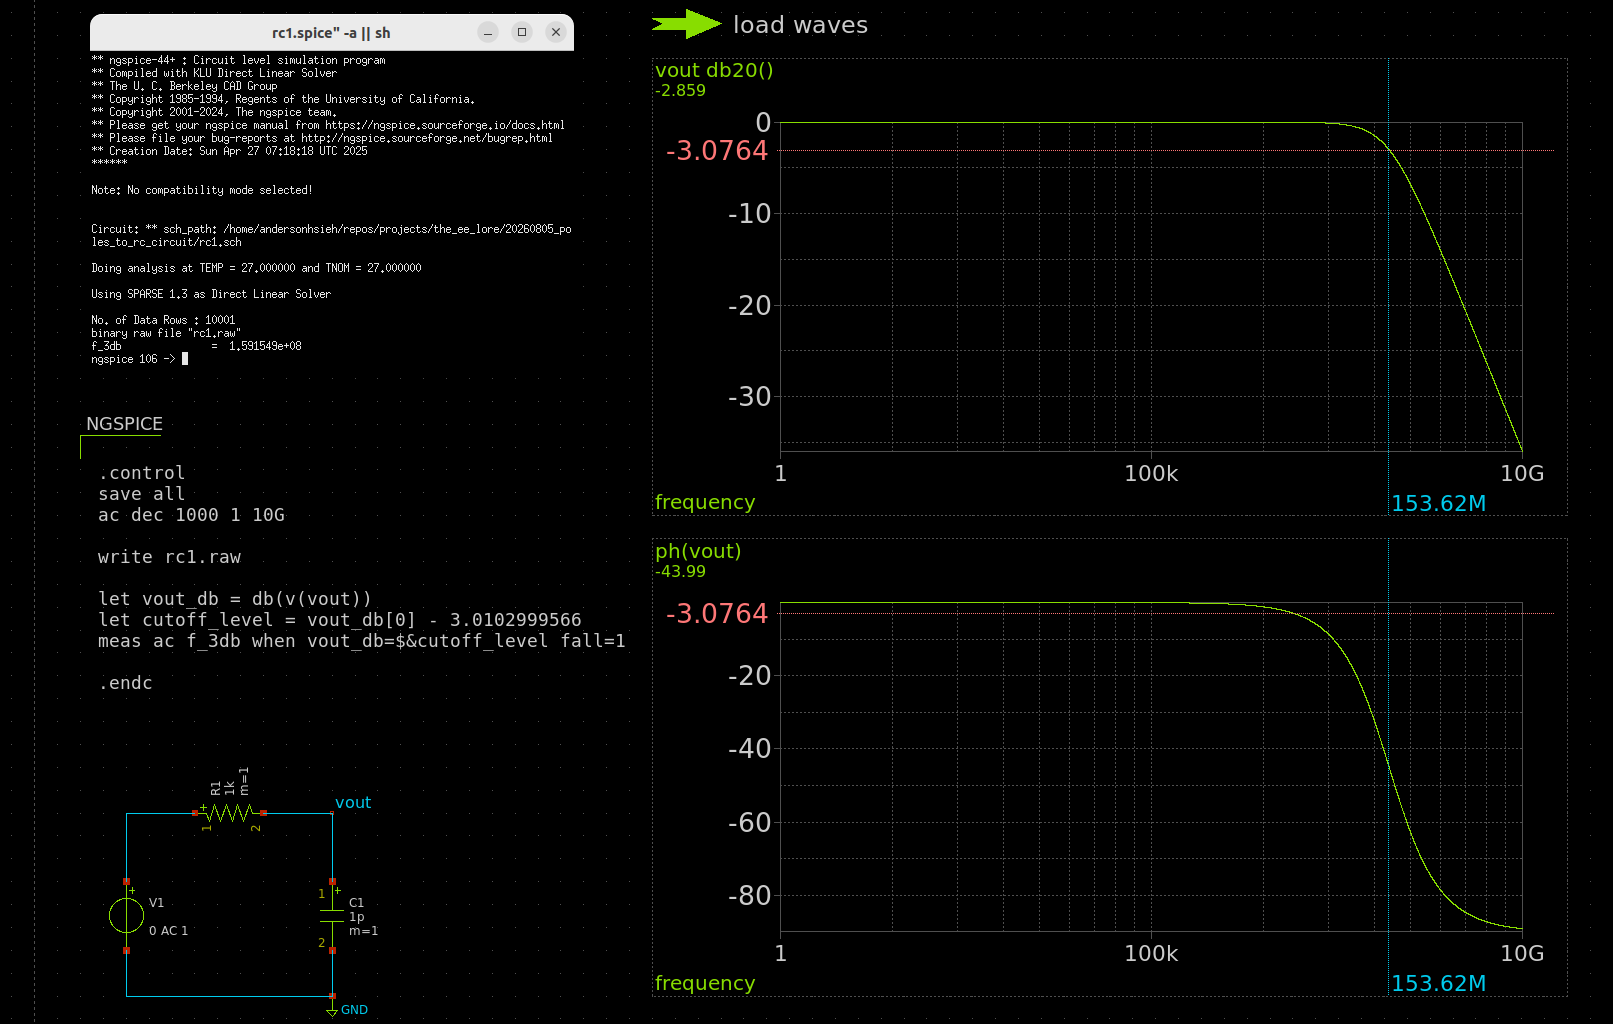
\includegraphics[width=\textwidth]{images/rc1_spice.png}
\section{Questions To Be Answered}
    \begin{enumerate}
        \item how do they tune VDD for ring oscillator in a real application?
        \item poles and zeros in oscillators
        \item current mirrors in differential ring oscillator
    \end{enumerate}
\section{Some Picture}

\appendix

\section{Derivation of the -3dB Voltage Ratio}
\label{app:minus-3db}
    For a purely resistive load,

    \begin{align*}
        P_{\text{load, avg}}
        &= \frac{V_{\text{out,rms}}^2}{R_{\text{load}}}.
    \end{align*}

    at -3dB cut off frequency, power delivered to a load with resistance R drops to half.
    \begin{align*}
        \frac{P_{\mathrm{current}}}{P_{\mathrm{max}}}&= \frac{1}{2} \\
        \frac{P_{\mathrm{current}}}{P_{\mathrm{max}}}&= \frac{1}{2} \\
        \left(\frac{V_{\mathrm{current}}}{V_{\mathrm{max}}}\right)^2&= \frac{1}{2} \\
        \frac{V_{\mathrm{current}}}{V_{\mathrm{max}}}&= \sqrt{\frac{1}{2}} \\
            &= \frac{1}{\sqrt{2}} \\
            &\approx 0.7071
    \end{align*}

\section{Why Use $V_{\mathrm{rms}}$ When Calculating Average Power?}
\label{app:why_vrms}
    RMS voltage is used because it represents the DC voltage that would
    produce the same average power, or heating, in a resistor.

    The instantaneous power dissipated by a resistor is
    \begin{align*}
        p(t) = \frac{v(t)^2}{R}.
    \end{align*}

    For a sinusoidal voltage,
    \begin{align*}
        v(t) = V_{\mathrm{peak}}\cos(\omega t),
    \end{align*}
    so the instantaneous power is
    \begin{align*}
        p(t) = \frac{V_{\mathrm{peak}}^2\cos^2(\omega t)}{R}.
    \end{align*}

    Since the average value of $\cos^2(\omega t)$ over one complete cycle
    is $1/2$, the average power is
    \begin{align*}
        P_{\mathrm{avg}} = \frac{V_{\mathrm{peak}}^2}{2R}.
    \end{align*}

    But if whenever we want to calucalte average power we gotta divide by 2 it's too much work, so to make it easier when calcualting average power over a complete cycle of a sinuosidal signal, we define a new kind of voltage, the RMS voltage

    The RMS voltage of a sine wave is
    \begin{align*}
        V_{\mathrm{rms}} = \frac{V_{\mathrm{peak}}}{\sqrt{2}}.
    \end{align*}
    Therefore, when we want to find average power of a sinsuoidal signal we can just divide the peak voltage by $\sqrt{2}$ and plug that into the power = I*V equation
    \begin{align*}
        P_{\mathrm{avg}} = \frac{V_{\mathrm{rms}}^2}{R}.
    \end{align*}

    For example, a sine wave with a peak voltage of \SI{1}{\volt} has an
    RMS voltage of approximately \SI{0.7071}{\volt}. Across a
    \SI{1}{\ohm} resistor, its average power is
    \begin{align*}
        P_{\mathrm{avg}}
        &= \frac{(\SI{0.7071}{\volt})^2}{\SI{1}{\ohm}} \\
        &\approx \SI{0.5}{\watt}.
    \end{align*}

    Thus, an AC voltage of \SI{0.7071}{\volt} RMS produces the same average
    heating in a resistor as if there is a a DC voltage of \SI{0.7071}{\volt} across the resistor.

\end{document}
